\documentclass[GTSResumen.tex]{subfiles}
%\usepackage{amsmath,amssymb}
%\usepackage[utf8]{inputenc}
%\usepackage[spanish]{babel}
%\usepackage[]{graphicx,wrapfig}
%\usepackage{enumerate}
%\usepackage{amsthm}
%\usepackage{tikz-cd}  
%\usetikzlibrary{babel} 
%\usepackage{pgf,tikz}
%\usepackage{mathrsfs}
%\usetikzlibrary{arrows}
%\usetikzlibrary{cd}    
%\usepackage[spanish]{babel}
%\usepackage{fancyhdr}
%\usepackage{titlesec}
%\usepackage{floatrow}    
%\usepackage{makeidx}      
%\usepackage[tocflat]{tocstyle}  
%\usetocstyle{standard} 
%%\usepackage{breqn}
%\usepackage{bm}         
%%\usepackage[sc]{mathpazo}
%%\usepackage{blindtext}
%\usepackage{color}   %May be necessary if you want to color links
%\usepackage{hyperref}
%\hypersetup{colorlinks=true,citecolor=red, linkcolor=blue}
%
%
%\renewcommand{\baselinestretch}{1,4}
%\setlength{\oddsidemargin}{0.25in}
%\setlength{\evensidemargin}{0.25in}
%\setlength{\textwidth}{6in}
%\setlength{\topmargin}{0.1in}
%\setlength{\headheight}{0.1in}
%\setlength{\headsep}{0.1in}
%\setlength{\textheight}{8in}
%\setlength{\footskip}{0.75in}
%
%\newtheorem{teorema}{Teorema}[section]
%\newtheorem{defi}[teorema]{Definición}
%\newtheorem{coro}[teorema]{Corolario}
%\newtheorem{lemma}[teorema]{Lema}
%\newtheorem{ej}[teorema]{Ejemplo}
%\newtheorem{ejs}[teorema]{Ejemplos}
%\newtheorem{observacion}[teorema]{Observación}
%\newtheorem{observaciones}[teorema]{Observaciones}
%\newtheorem{prop}[teorema]{Proposición}
%\newtheorem{propi}[teorema]{Propiedades}
%\newtheorem{nota}[teorema]{Nota}
%\newtheorem{notas}[teorema]{Notas}
%\newtheorem*{dem}{Demostración}
%\newtheorem{ejer}[teorema]{Ejercicio}
%\newtheorem{consec}[teorema]{Consecuencia}
%\newtheorem{consecs}[teorema]{Consecuencias}
%
%\providecommand{\abs}[1]{\lvert#1\rvert}
%\providecommand{\norm}[1]{\lVert#1\rVert}
%\providecommand{\ninf}[1]{\norm{#1}_\infty}
%\providecommand{\numn}[1]{\norm{#1}_1}
%\providecommand{\gabs}[1]{\left|{#1}\right|}
%\newcommand{\bor}[1]{\mathcal{B}(#1)}
%\newcommand{\R}{\mathbb{R}}
%\newcommand{\Z}{\mathbb{Z}}
%\newcommand{\N}{\mathbb{N}}
%\newcommand{\Q}{\mathbb{Q}}
%\newcommand{\C}{\mathbb{C}}
%\newcommand{\Pro}{\mathbb{P}}
%\newcommand{\Tau}{\mathcal{T}}
%\newcommand{\verteq}{\rotatebox{90}{$\,=$}}
%\newcommand{\vertequiv}{\rotatebox{110}{$\,\equiv$}}
%\providecommand{\lrg}{\longrightarrow}
%\providecommand{\func}[2]{\colon{#1}\longrightarrow{#2}}
%\newcommand*{\QED}{\hfill\ensuremath{\blacksquare}}
%\renewcommand*\circled[1]{\tikz[baseline=(char.base)]{
%            \node[shape=circle,draw,inner sep=1.5pt] (char) {#1};}}
%\renewcommand*{\longhookarrow}{\ensuremath{\lhook\joinrel\relbar\joinrel\rightarrow}}
%
%\newenvironment{solucion}{\begin{trivlist}
%\item[\hskip \labelsep {\textit{Solución}.}\hskip \labelsep]}{\end{trivlist}}
%
%\def\quot#1#2{%
%    \raise1ex\hbox{$#1$}\Big/\lower1ex\hbox{$#2$}%
%}
%
%\makeatletter
%\renewcommand\tableofcontents{%
%  \null\hfill\textbf{\Large\contentsname}\hfill\null\par
%  \@mkboth{\MakeUppercase\contentsname}{\MakeUppercase\contentsname}%
%  \@starttoc{toc}%
%}
%
%\pagestyle{fancy}
%\fancyhf{}
%\rhead{Topología de Superficies (Grado en Matemáticas)}
%\lhead{Curso 2016/2017}
%\cfoot{\thepage}
\begin{document}
%
\renewcommand\chaptername{\Huge Tema}
%
\titleformat{\chapter}[display]
    {\normalfont\huge\bfseries}{\chaptertitlename\ \thechapter}{10pt}{\Huge}
\titlespacing*{\chapter}{0pt}{-1cm}{10pt}
%
%
%
%\tableofcontents


\setcounter{chapter}{4}

\chapter{Teorema de Seifert-Van Kampen}
\section{Presentación de grupos.\\ Teorema de Seifert-Van Kampen}
\begin{defi}
Sea $G$ un grupo. Se llama \textbf{presentación} de $G$ a un par $\langle S|R\rangle$ donde $S$ es un conjunto de generadores (esto es, todo elemento de $G$ se puede escribir como un producto de elementos y sus inversos de $S\subseteq G$). Los productos de elementos de $S$ (y sus inversos) se llaman \textbf{palabras} de $S$.\\
Por su parte, $R$ es un conjunto de palabras de $S$ que son iguales al elemento neutro $e\in G$, las palabras en $R$ se llaman \textbf{relaciones} de $G$. Además, el conjunto $R$ es elegido para que si dos palabras $p_1$ y $p_2$ de $S$ representan el mismo elemento de $G$, entonces se puede pasar de una a otra por operaciones deducidas a partir de las igualdades $r^{\pm1} = e$ con $r\in R$ y las relaciones obvias del grupo $G$. \\
En el caso particular de que $R=\emptyset$, se dice que $\langle S|\emptyset\rangle$ es un \textbf{grupo libre} con base $S$.
\end{defi}

\begin{nota}
En la presentación del grupo no se suelen incluir relaciones triviales como, por ejemplo, $aa^{-1}=e$, que se suponen dadas implícitamente por la estructura del grupo.
\end{nota}

\begin{nota}[Importante] Obsérvese que, dado un grupo $H$, para determinar que una aplicación $f\func{G=\langle S|R\rangle}{H}$ es un homomorfismo de grupos bastará comprobar que $f(s^{-1})=f(s)^{-1}$ y $f(s_1^{\pm 1}\cdot s_2^{\pm 1})=f(s_1)^{\pm 1}\cdot f(s_2)^{\pm 1}$ para $s,s_1,s_2\in S$, y que los elementos de $R$ van todos al neutro de $H$. En efecto, cualquier $g\in G$ puede ser escrito como $g=s_1^{\pm 1}\cdots s_m^{\pm 1}$ con $s_i\in S$. Entonces $f(g)=f(s_1)^{\pm 1}\cdots f(s_m)^{\pm 1}$ no depende de la palabra de $S$ elegida para representar $g$, de pues si $g$ puede ser representado por otra palabra de $S$, las transformaciones por medio de elementos de $R$ (sus inversos y las relaciones triviales de $G$) se corresponden por $f$ con operar con el elemento neutro, por lo que las dos posibles imágenes por $f$ de las dos palabras que representan a $g$ son coincidentes.
\end{nota}
\begin{comment}
\begin{ej} Algunos ejemplos de presentaciones son:
\begin{enumerate}
\item $\Z\begin{cases}
\langle a|\ \rangle  \text{ grupo libre de base }\{a\}\\
\langle a,b|ab^{-1}\rangle
\end{cases}\quad$ Son presentaciones equivalentes.
\item $\Z_n: \langle a| a^n\rangle$.
\item $\Z\times\Z: \langle a,b| aba^{-1}b^{-1}\rangle$. En este caso $R$ expresa la commutatividad, que no se considera relación trivial, ya que trabajamos con grupos no necesariamente abelianos. Nótese que además $R$ coincide con la identificación de las aristas en el polígono fundamental del toro.
\item $\Z\underbrace{\times\cdots\times}_{n\ veces}\Z: \langle a_1,\dots,a_n|a^{}_i a^{}_j a^{-1}_i a^{-1}_j\ 1\leq i\leq j\leq n\rangle$. Más generalmente, una presentación del grupo abeliano finitamente generado  $A=\Z^n\times\Z_{n_1}\times\cdots\times\Z_{n_k}$ es 
\begin{gather*}
\langle a_1,\dots,a_n,b_1,\dots,b_k|\ b^{n_s}_s,\ a^{}_ia^{}_ja^{-1}_ia^{-1}_j,\ a^{}_j b^{}_s a^{-1}_j b^{-1}_s,\ 1\leq i,j\leq n, 1\leq s\leq k\rangle.
\end{gather*}
\end{enumerate}
\end{ej}
\end{comment}
\begin{defi}
Sea $G$ un grupo con presentación $\langle S|R\rangle$. Se llama \textbf{abelianización} de $G$ al grupo abeliano $G^{ab}$ con presentación $\langle S| R\cup R_{ab}\rangle$ donde $R_{ab}=\{s^{}_i s^{}_j s^{-1}_i s^{-1}_j,\ s^{}_i, s^{}_j\in S \}$. Las expresiones $s^{}_i s^{}_j s^{-1}_i s^{-1}_j$ se suelen abreviar como $[s_i,s_j]$, lo que se conoce como \textbf{conmutador} de $s_i$ y $s_j$.
\end{defi}

\begin{ej}\
$\Z=\langle a|\ \rangle\Rightarrow \Z^{ab}=\langle a| aaa^{-1}a^{-1}\rangle=\langle a|\ \rangle =\Z$. En general, si $A$ es abeliano $A^{ab}=A$. En particular $(\Z^n)^{ab}=\Z^n$.
\end{ej}

\begin{defi}
Sean $G_1=\langle S_1|R_1\rangle$ y $G_2=\langle S_2|R_2\rangle$ dos grupos disjuntos con elementos neutros $e_1$ y $e_2$. Se llama \textbf{producto libre} de $G_1$ y $G_2$ al grupo denotado $G_1*G_2$ con presentación
\[
\langle S_1\cup S_2|R_1\cup R_2\cup\{e_1,e_2\}\rangle.
\]
Esto es, se identifican los elementos neutros de $G_1$ y $G_2$ con el de $G_1*G_2$ y se opera en $G_1*G_2$ con las relaciones de $G_1$ y $G_2$ por separado, de manera que solo se fusionan elementos de $G_1$ o elementos de $G_2$ no nulos de los grupos originales.
\end{defi}

\begin{nota}\
\begin{enumerate}
\item Habitualmente se presupone que los elementos neutros son el mismo y se escribe simplemente $\langle S_1\cup S_2|R_1\cup R_2\rangle$ para la presentación de $G_1*G_2$.
\item Dados dos grupos $G$ y $H$ siempre se pueden encontrar grupos isomorfos disjuntos:

Sea $G'=G\times\{0\}$ con la operación $(g,0)\cdot(g',0)=(gg',0)$ y $H'=H\times\{1\}$ con la operación análoga $(h,1)\cdot(h',1)=(hh',1)$.
\item Obsérvese que hay definidos unos homomorfismos inyectivos $k_i\func{G_i}{G_1*G_2}\quad k_i(g)=g$ para cada $g\in G_i$. Más aún, dos homomorfismos cualesquiera $h_1\func{G_1}{H}$ y $h_2\func{G_2}{H}$, llegando al mismo grupo $H$ determinan un homomorfismo $h\func{G_1*G_2}{H}$ por $h(g_i)=h_i(g_i)$ y por tanto $h_i=h\circ k_i\ (i=1,2)$.
\end{enumerate}
\end{nota}
\begin{comment}
\begin{ej}\
\begin{enumerate}
\item $\Z\underbrace{*\cdots *}_{n\ veces}\Z: \langle a_1,\dots,a_n|\ \rangle$. Grupo libre con base $a_1,\dots,a_n$.
\item $\Z*\Z_2: \langle a,b|b^2\rangle$.
\item $\Z_n*\Z_m: \langle a,b| a^n,b^m\rangle$.
\item $(G_1*G_2)^{ab}=G_1^{ab}\times G_2^{ab}$. 
\end{enumerate}
\end{ej}
\end{comment}
El producto libre es un caso particular de la siguiente construccción.  

\begin{defi}
Sea el siguiente diagrama de homorfismos de grupos:
\[
\begin{tikzcd}
G_0 \ar[r, "f_1"]\arrow[d,"f_2 "'] & G_1\\
G_2
\end{tikzcd}
\]
donde $G_i$ tiene presentación $\langle S_i|R_i\rangle$ ($i=0,1,2$). Se llama \textbf{producto amalgamado} del diagrama del grupo $G$ con presentación
\[
\langle S_1\cup S_2 | R_1\cup R_2\cup R_{12}\rangle
\]
con $R_{12}=\{f^{}_1(s)f^{}_2(s)^{-1},\ s\in S_0\}$, esto es, $f_1(s)=f_2(s)$ en $G$. Es decir, el producto amalgamado es el resultado de introducir las relaciones $R_{12}$ en el producto libre $G_1*G_2$.
\end{defi}

\begin{nota}[Importante] Todo diagrama conmutativo de grupos
\[
\begin{tikzcd}
\langle S_0|R_0\rangle =G_0 \ar[r, "f_1"]\arrow[d,"f_2 "'] & G_1=\langle S_1|R_1\rangle\ar[d,dashed,"f'_1"]\\
\langle S_2|R2 \rangle =G_2\ar[r, dashed, "f'_2"'] & H
\end{tikzcd}
\]
induce un homomorfismo $\varphi\func{G}{H}$ donde $G=\langle S_1\cup S_2 | R_1\cup R_2\cup R_{12}\rangle$ es el producto amalgamado del diagrama con flechas en línea continua. El homomorfismo inducido está definido como $\varphi(s_i)=f'_i(s_i)$ para $s_i\in S_i$ ($i=1,2$) pues, por ser $f'_i$ homomorfismo, $f'_i(R_i)=e\in H$ y por la conmutatividad del diagrama, para todo $s\in S_0$
\[
\varphi(f_1(s)f_2(s)^{-1})=f'_1f_1^{}(s)f'_2f_2^{}(s)^{-1}=e\in H;
\]
así pues, $\varphi(R_{12})=e\in H$.
\end{nota}

\begin{ej} Tres casos particulares de interés:
\begin{enumerate}
\item Si $G_0=\{1\}$, el producto amalgamado es $G_1*G_2$.
\item Si $G_0$ es cualquiera y $G_1=G_2=\{1\}=\langle\ |\ \rangle$, el producto amalgamado vuelve a ser el grupo trivial $\{1\}=\langle\ |\ \rangle$.
\item Si $G_2=\{1\}$ y $f\func{G_0}{G_1}$ es sobreyectivo, entonces el producto amalgamado es también el grupo trivial. Ejercicio.
\end{enumerate}

\end{ej}

%\vspace{0.5cm}

\begin{teorema}[\textbf{Teorema de Seifert-Van Kampen}]\label{SVK} Sea $X$ un espacio topológico tal que $X=X_1\cup X_2$ con $X_1, X_2$ abiertos y $X_1\cap X_2$ conexo por caminos. Entonces, si $x_0\in X_1\cap X_2$ tenemos el diagrama conmutativo de grupos
\[
\begin{tikzcd}
\pi_1(X_1\cap X_2,x_0) \ar[r, "i_{1*}"]\arrow[d,"i_{2*} "'] & \pi_1(X_1,x_0)\ar[d,dashed,"j_{1*}"]\\
\pi_1(X_2,x_0)\ar[r,dashed,"{j_2}*"'] & \pi_1(X,x_0)
\end{tikzcd}
\]
donde
\begin{gather*}
X_1\cap X_2\overset{i_1}{\longhookarrow} X_1\overset{j_1}{\longhookarrow} X\\
X_1\cap X_2\overset{i_2}{\longhookarrow} X_2\overset{j_2}{\longhookarrow} X
\end{gather*}
son las correspondientes inclusiones. Bajo estas hipótesis, $\pi_1(X,x_0)$ es isomorfo al producto amalgamado del diagrama de flechas en trazo continuo  $G$.\\
Más aún, el homomorfismo $\varphi\func{G}{\pi_1(X,x_0)}$ inducido por $j_{1*}\func{\pi_1(X_1,x_0)}{\pi_1(X,x_0)}$ y $j_{2*}\func{\pi_1(X_2,x_0)}{\pi_1(X,x_0)}$ es un isomorfismo.
\end{teorema}
\begin{comment}
{\bf Idea del teorema:}
Sea $\alpha\func{I}{X}$ un lazo en $x_0$ que es la yuxtaposición de un camino $\alpha_{\big|[0,t_1]}$ en $X_1$ y otro $\alpha_{\big|[t_1,1]}$ en $X_2$. Consideramos $\gamma$ un camino en $X_1\cap X_2$ entre $x_0=\alpha(0)=\alpha(1)$ y $x_1=\alpha(t_1)$. Ahora $\alpha$ puede descomponerse como yuxtaposición de dos lazos
\[
\underbrace{(\alpha_{\big|[0,t_1]}*\overline{\gamma})}_{\text{En }X_1}*\underbrace{(\gamma*\alpha_{\big|[t_1,1]})}_{\text{En }X_2}
\]
el primero en $j_{1*}(\pi_1(X_1,x_0))$ y el otro en $j_{2*}(\pi_1(X_2,x_0))$.

\begin{figure}[h!]
	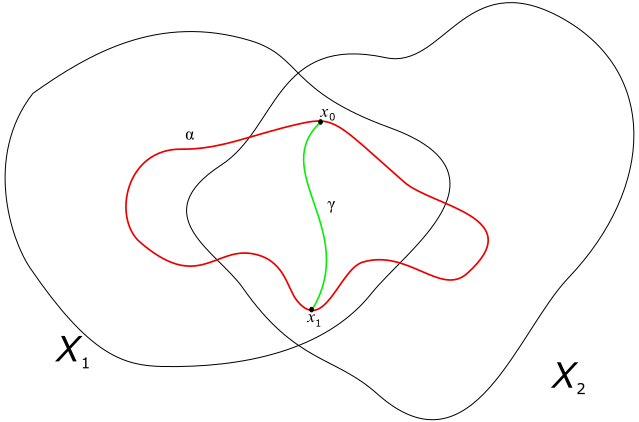
\includegraphics[scale=0.4]{text4180}
\end{figure}\

Para una prueba completa consultar \cite{Hatcher}.

\newpage
\end{comment}
\subsection{Uso del teorema de Seifert-Van Kampen}

A partir del Teorema de Seifert-Van Kampen es posible obtener una presentación explícita del grupo fundamental $\pi_1(X,x_0)$ siguiendo el siguiente procedimiento.

$\circled{1}$ Si $\pi_1(X_1\cap X_2)=\langle S_0|R_0\rangle$ y $\pi_1(X_i,x_0)=\langle S_i|R_i\rangle$ ($i=1,2$) entonces sabemos que el producto amalgamado $G$ del diagrama
\[
\begin{tikzcd}
\pi_1(X_1\cap X_2,x_0) \ar[r, "i_{1*}"]\arrow[d,"i_{2*} "'] & \pi_1(X_1,x_0)\\
\pi_1(X_2,x_0)
\end{tikzcd}
\]
tiene presentación $\langle S_1\cup S_2 | R_1\cup R_2\cup R_{12}\rangle$.

$\circled{2}$ En las relaciones $i_{1*}(s)i_{2*}(s)^{-1}$ de $R_{12}$, donde $s\in S_0$, se busca cómo expresar $i_{1*}(s)$ e $i_{2*}(s)$ en función de los generadores en $S_1$ y $S_2$ respectivamente. Una vez hecho esto, todas las relaciones de $R_1\cup R_2\cup R_{12}$ estarán escritas explícitamente con los elementos de $S_1\cup S_2$.

$\circled{3}$ Como $\varphi\func{G}{\pi_1(X,x_0)}$ es un isomorfismo, teniendo en cuenta la definición de $\varphi$, $\pi_1(X,x_0)$ tiene como presentación a
\[
\langle\varphi(S_1)\cup\varphi(S_2)|\ \varphi(R_1)\cup\varphi(R_2)\cup\varphi(R_{12})\rangle=\langle j_{1*}(S_1)\cup j_{2*}(S_1)|\ j_{1*}(R_1)\cup j_{2*}(R_2)\cup\varphi(R_{12})\rangle
\]

$\circled{4}$ Finalmente, un elemento $s\in S_k$ ($k=1,2$) es la clase de un lazo $\alpha$ en $X_k$ basado en $x_0$, por tanto $j_{k*}(\alpha)$ es la clase de ese mismo lazo $\alpha$ pero ahora en $X$, ya que  $j_{k*}[\alpha]=[j_k\circ\alpha]$. Análogamente, cualquier relación $r\in R_k$ es un producto de clases de lazos en $X_k$ basados en $x_0$, por tanto, como $j_{k*}$ es homomorfismo, $j_{k*}(r)$ es un producto de las clases de esos mismos lazos pero ahora en $X$.

$\circled{5}$ Por último, cada relación $i_{1*}(s)i_{2*}(s)^{-1}\in R_{12}$ ($s\in S_0$), que ya tenemos escrita como un producto de elementos de $S_1\cup S_2$, se transforma por $\varphi$ en un producto de imágenes por $j_{1*}$ y $j_{2*}$ de esos elementos (por $j_{1*}$ si el elemento es de $S_1$ y por $j_{2*}$ si está en $S_2$). Así pues, las relaciones en $\varphi(R_{12})$ son ahora productos de elementos de $j_{1*}(S_1)\cup j_{2*}(S_2)$ que, recordemos, eran las clases en $X$ de los lazos que representaban a los elementos de $S_1\cup S_2$.


\begin{comment}
\begin{ej}\
\begin{itemize}
\item[$\circled{1}$]$\bm{\pi_1(S^2,x_0)}$


\begin{tikzpicture}[line cap=round,line join=round,>=triangle 45,x=1.0cm,y=1.0cm]
\clip(-3.480326366784244,-2) rectangle (6.657414680047705,2.);
\draw(0.,0.) circle (2.cm);
\draw [rotate around={0.:(0.00465710259671068,0.)}] (0.00465710259671068,0.) ellipse (1.995808730496537cm and 0.6394069228671712cm);
\draw [rotate around={0.:(0.013387632714876802,1.2940236202234447)},dash pattern=on 2pt off 2pt] (0.013387632714876802,1.2940236202234447) ellipse (1.4788951435192086cm and 0.3901781077494605cm);
\draw [rotate around={0.:(0.013387632714876785,-1.2940236202234447)},dash pattern=on 2pt off 2pt] (0.013387632714876785,-1.2940236202234447) ellipse (1.4800281280478624cm and 0.394450719425271cm);
\draw (-2.5,1.3485189871155068)-- (-2.5,-1.9278546667788097);
\draw (-2.5,1.3485189871155068)-- (-2.0125577717429226,1.3485189871155068);
\draw (-2.5,-1.9278546667788097)-- (-2.0125577717429226,-1.9278546667788095);
\draw (1.99994684931873,-1.4271384133352825)-- (2.5,-1.4271384133352825);
\draw (2.5,-1.4271384133352825)-- (2.5,1.913908418620639);
\draw (2.5,1.913908418620639)-- (1.99994684931873,1.913908418620639);
\draw (-3.2,0.02740704121017147) node[anchor=north west] {$X_1$};
\draw (2.6,0.6) node[anchor=north west] {$X_2$};
\end{tikzpicture}

Tal como lo hemos elegido, $X_1\cap X_2$ es conexo por caminos y tiene al ecuador como retracto de deformación fuerte, por lo que $\pi_1(X_1\cap X_2,x_0)\cong\pi_1(S^1,x_0)\cong\Z$. Por otro lado, tanto $X_1$ como $X_2$ son homeomorfos a un disco abierto, que es contráctil, luego $\pi_1(X_1,x_0)=\pi_1(X_2,x_0)=\{1\}$. El teorema de Seifert-Van Kampen (\ref{SVK}) nos da el siguiente diagrama
\[
\begin{tikzcd}
\pi_1(X_1\cap X_2,x_0)\cong\Z \ar[r, ""]\arrow[d,""'] & \pi_1(X_1,x_0)=\{1\}\arrow[d,dashed]\\
\pi_1(X_2,x_0)=\{1\}\arrow[r,dashrightarrow] & \pi_1(S^2,x_0)=\{1\}
\end{tikzcd}
\]
Por lo tanto, el grupo fundamental de $S^2$ es el grupo trivial.


\item[$\circled{2}$]$\bm{\pi_1(S^1\vee S^1,x_0)}$

\begin{tikzpicture}[line cap=round,line join=round,>=triangle 45,x=1.0cm,y=1.0cm]
\clip(-4.132863999999993,-4.614538666666662) rectangle (8.133802666666664,1.326794666666668);
\draw(-1.,0.) circle (1.cm);
\draw(1.,0.) circle (1.cm);
\draw(-3.,-3.) circle (1.cm);
\draw(3.,-3.) circle (1.cm);
\draw [shift={(-1.,-3.)}] plot[domain=1.5707963267948966:4.71238898038469,variable=\t]({1.*1.*cos(\t r)+0.*1.*sin(\t r)},{0.*1.*cos(\t r)+1.*1.*sin(\t r)});
\draw [shift={(1.,-3.)}] plot[domain=-1.5707963267948966:1.5707963267948966,variable=\t]({1.*1.*cos(\t r)+0.*1.*sin(\t r)},{0.*1.*cos(\t r)+1.*1.*sin(\t r)});
\draw [->] (-1.5546666666666642,-1.0653333333333301) -- (-2.,-2.);
\draw [->] (1.592,-0.9906666666666636) -- (2.,-2.);
\draw (-3.2,1) node[anchor=north west] {$S^1\vee S^1$};
\draw (-4.3,-1.8092053333333302) node[anchor=north west] {$X_1$};
\draw (3.8,-1.8518719999999969) node[anchor=north west] {$X_2$};
\draw [shift={(6.,-3.)}] plot[domain=-1.5707963267948966:1.5707963267948966,variable=\t]({1.*1.*cos(\t r)+0.*1.*sin(\t r)},{0.*1.*cos(\t r)+1.*1.*sin(\t r)});
\draw [shift={(8.,-3.)}] plot[domain=1.5707963267948966:4.71238898038469,variable=\t]({1.*1.*cos(\t r)+0.*1.*sin(\t r)},{0.*1.*cos(\t r)+1.*1.*sin(\t r)});
\draw (6.3,-1.5212053333333304) node[anchor=north west] {$X_1\cap X_2$};
\end{tikzpicture}

En este caso, $X_1\cap X_2$ es contráctil, por lo que $\pi_1(X_2\cap X_2,x_0)=\{1\}$. Por otro lado, tanto $X_1$ como $X_2$ tienen a $S^1$ como retracto de deformación fuerte, por lo que las inclusiones $k_1\func{S^1}{X_1}$ y $k_1\func{S^1}{X_2}$ inducen isomorfismos $k_{1*}\func{\pi_1(S^1,x_0)}{\pi_1(X_1,x_0)}$ y $k_{2*}\func{\pi_1(S^1,x_0)}{\pi_1(X_2,x_0)}$. Por tanto, $\pi_1(X_1,x_0)=\pi_1(X_2,x_0)\cong\Z$, siendo los generadores las clases $\varepsilon_i \in \pi_1(X_i,x_0)$ de las vueltas canónicas $t\mapsto e^{2\pi it}$ de las circunferencias completas de $X_1$ y $X_2$, respectivamente. El diagrama resultante del teorema de Seifert-Van Kampen (\ref{SVK}) es el siguiente
\[
\begin{tikzcd}
\pi_1(X_1\cap X_2,x_0)\cong\{1\} \ar[r, "i_1*"]\arrow[d,"i_2*"'] & \pi_1(X_1,x_0)=\langle\varepsilon_1|\ \rangle\arrow[d,dashed,"j_1*"]\\
\langle\varepsilon_2|\ \rangle =\pi_1(X_2,x_0)\arrow[r,dashrightarrow,"j_2*"'] & \pi_1(S^1\vee S^1,x_0)=\langle j_{1*}(\varepsilon_1), j_{2*}(\varepsilon_2)|\ \rangle
\end{tikzcd}
\]
El resultado es el grupo libre con dos generadores que son las clases en $\pi_1(S^1\vee S^1,x_0)$ de las vueltas canónicas de las dos circunferencias que componen $S^1\vee S^1$. Nótese que no es abeliano.

En general $\pi_1(S^1\vee\cdots\vee S^1,x_0)\cong\Z*\cdots *\Z$, donde $S^1\vee\cdots\vee S^1$ es el resultado de unir una cantidad finita de circunferencias por un solo punto común a todas.



\item[$\circled{3}$]$\bm{\pi_1(T,x_0)}$ (Toro)

\definecolor{ffffff}{rgb}{1.,1.,1.}
\definecolor{zzttqq}{rgb}{0.6,0.2,0.}
\begin{tikzpicture}[line cap=round,line join=round,>=triangle 45,x=1.0cm,y=1.0cm]
\clip(-1.6541333333333335,-1.6) rectangle (9.140533333333332,2.6);
\fill[color=zzttqq,fill=zzttqq,fill opacity=0.2] (0.,0.) -- (1.,0.) -- (1.,1.) -- (0.,1.) -- cycle;
\fill[color=zzttqq,fill=zzttqq,fill opacity=0.2] (2.,-1.5) -- (3.,-1.5) -- (3.,-0.5) -- (2.,-0.5) -- cycle;
\draw [color=ffffff,fill=ffffff,fill opacity=1.0] (2.5,-1.) circle (0.20010805969664447cm);
\draw [line width=0.4pt,color=zzttqq,fill=zzttqq,fill opacity=0.2] (5.,0.5) circle (0.45cm);
\draw [line width=0.4pt] (5.,0.5) circle (0.35cm);
\draw [color=ffffff,fill=ffffff,fill opacity=1.0] (5.,0.5) circle (0.17782688210729017cm);
\draw [line width=0.4pt,color=zzttqq,fill=zzttqq,fill opacity=0.2] (2.5,1.5) circle (0.45cm);
\draw [color=zzttqq] (0.,0.)-- (1.,0.);
\draw [color=zzttqq] (1.,0.)-- (1.,1.);
\draw [color=zzttqq] (1.,1.)-- (0.,1.);
\draw [color=zzttqq] (0.,1.)-- (0.,0.);
\draw [->] (5.,-0.5) -- (5,0.15);
\draw [->] (0.,1.) -- (0.6,1.);
\draw [->] (0.,0.) -- (0.6,0.);
\draw [->] (0.,0.) -- (0.,0.6);
\draw [->] (1.,0.) -- (1.,0.6);
\draw [->] (2.,-0.5) -- (2.6,-0.5);
\draw [->] (2.,-1.5) -- (2.6,-1.5);
\draw [->] (2.,-1.5) -- (2,-0.9);
\draw [->] (3.,-1.5) -- (3,-0.9);
\draw [->] (1.780533333333333,1.3104) -- (1.2429333333333332,0.9946666666666657);
\draw [->] (1.8146666666666664,-0.34506666666666636) -- (1.2856,0.);
\draw [color=zzttqq] (2.,-1.5)-- (3.,-1.5);
\draw [color=zzttqq] (3.,-1.5)-- (3.,-0.5);
\draw [color=zzttqq] (3.,-0.5)-- (2.,-0.5);
\draw [color=zzttqq] (2.,-0.5)-- (2.,-1.5);
\draw [->] (4.016266666666666,0.19253333333333317)--(3.3165333333333327,-0.2597333333333331);
\draw [->] (3.9992,0.9008)--(3.3165333333333327,1.3274666666666655);
\draw (1.8,2.5) node[anchor=north west] {$X_1=\text{disco abierto}$};
\draw (4.75,-0.5) node[anchor=north west] {$S^1$};
\draw (2.2,0) node[anchor=north west] {$X_2$};
\draw (0.1,-0.5) node[anchor=north west] {$\text{ Hacemos}$};
\draw (0.1,-0.8) node[anchor=north west] {$\text{un agujero}$};
\draw (5.5,0.74464) node[anchor=north west] {$X_1\cap X_2$};
\draw (-0.5,0.6) node[anchor=north west] {$a$};
\draw (1.1,0.6) node[anchor=north west] {$a$};
\draw (0.4,1.4) node[anchor=north west] {$b$};
\draw (0.4,0) node[anchor=north west] {$b$};
\draw (1.2,1.8) node[anchor=north west] {$j_1$};
\draw (1.5,0.3) node[anchor=north west] {$j_2$};
\draw (3.3,0.4) node[anchor=north west] {$i_1$};
\draw (3.5,1.6) node[anchor=north west] {$i_2$};
\end{tikzpicture}

Obsérvese que $X_1$ es contráctil, así que $\pi_1(X_1,x_0)=\{1\}$. Por otra parte, $X_1\cap X_2$ tiene a $S^1$ como retracto de deformación fuerte, por lo que $\pi_1(X_1\cap X_2,x_0)=\langle [\alpha^0]|\ \rangle\cong\Z$, siendo $\alpha^0(t)=e^{2\pi it}$ la vuelta canónica en $S^1$ y la clase es la de $\alpha^0$ en $\pi_1(X_1\cap X_2,x_0)$, ya que la inclusión $i\func{S^1}{X_1\cap X_2}$ induce un isomorfismo $i_*\func{\pi_1(S^1,x_0)}{\pi_1(X_1\cap X_2,x_0)}$. Vamos a ver con más detalle lo que le ocurre a $X_2$.

\definecolor{ffffff}{rgb}{1.,1.,1.}
\definecolor{zzttqq}{rgb}{0.6,0.2,0.}
\begin{tikzpicture}[line cap=round,line join=round,>=triangle 45,x=1.0cm,y=1.0cm]
\clip(-0.5,-0.4) rectangle (14.64,2.3);
\fill[color=zzttqq,fill=zzttqq,fill opacity=0.1] (0.,0.) -- (2.,0.) -- (2.,2.) -- (0.,2.) -- cycle;
\draw [line width=0.4pt,color=ffffff,fill=ffffff,fill opacity=1.0] (1.,1.) circle (0.40094333210013056cm);
\draw [color=zzttqq] (0.,0.)-- (2.,0.);
\draw [color=zzttqq] (2.,0.)-- (2.,2.);
\draw [color=zzttqq] (2.,2.)-- (0.,2.);
\draw [color=zzttqq] (0.,2.)-- (0.,0.);
\draw (1.,1.) circle (0.4009433321001305cm);
\draw (0.,0.)-- (0.7066666666666672,0.7266666666666661);
\draw [->] (2.48,0.9933333333333326) -- (5.,1.);
\draw (6.,0.)-- (8.,0.);
\draw (8.,0.)-- (8.,2.);
\draw (8.,2.)-- (6.,2.);
\draw (6.,2.)-- (6.,0.);
\draw (6.,0.)-- (7.,1.);
\draw (9.,0.)-- (10.,1.);
\draw (9.5,1.5) circle (0.7071067811865476cm);
\draw (10.5,0.5) circle (0.7071067811865476cm);
\draw [->] (0.,0.) -- (0.,1.);
\draw [->] (2.,0.) -- (2.,1.);
\draw [->] (0.,0.) -- (1.,0.);
\draw [->] (0.,2.) -- (1.,2.);
\draw [->] (6.,0.) -- (7.,0.);
\draw [->] (6.,2.) -- (7.,2.);
\draw [->] (6.,0.) -- (6.,1.);
\draw [->] (8.,0.) -- (8.,1.);
\draw [->] (10.,2.) -- (10.146162342755964,1.7871832634470939);
\draw [->] (11.,1.) -- (10.833123950447732,1.1237214391361718);
\draw (0.65,0.65) node[anchor=north west] {$x_0$};
\draw (0.2,1.6) node[anchor=north west] {$S^1$};
\draw (2.52,1.5) node[anchor=north west] {$\text{Se retrae con}$};
\draw (2.52,1.) node[anchor=north west] {$\text{deformación a}$};
\draw (8.493333333333336,1.02) node[anchor=north west] {$\cong$};
\draw (11.42666666666667,1.06) node[anchor=north west] {\large{$\equiv Y$}};
\draw (6.92,0.9) node[anchor=north west] {$x_0$};
\draw (8.986666666666668,0) node[anchor=north west] {$x_0$};
\draw (0.3,0.4) node[anchor=north west] {$\gamma$};
\draw (6.52,0.54) node[anchor=north west] {$\gamma$};
\draw (9.3,0.4) node[anchor=north west] {$\gamma$};
\draw (9.48,2.2066666666666648) node[anchor=north west] {$a$};
\draw (10.693333333333335,0.9666666666666653) node[anchor=north west] {$b$};
\draw (-0.41,1.1933333333333318) node[anchor=north west] {$a$};
\draw (2.,1.22) node[anchor=north west] {$a$};
\draw (0.8933333333333339,2.4333333333333313) node[anchor=north west] {$b$};
\draw (0.88,0.02) node[anchor=north west] {$b$};
\draw (5.573333333333334,1.18) node[anchor=north west] {$a$};
\draw (8.08,1.113333333333332) node[anchor=north west] {$a$};
\draw (6.9333333333333345,-0.02) node[anchor=north west] {$b$};
\draw (7.08,2.3933333333333313) node[anchor=north west] {$b$};
\draw (9.986666666666668,1.02) node[anchor=north west] {$x_1$};
\draw (-0.5,0) node[anchor=north west] {$x_1$};
\draw (-0.5,2) node[anchor=north west] {$x_1$};
\draw (2,2) node[anchor=north west] {$x_1$};
\draw (2,0) node[anchor=north west] {$x_1$};
\draw (5.5,0) node[anchor=north west] {$x_1$};
\draw (5.5,2) node[anchor=north west] {$x_1$};
\draw (8,2) node[anchor=north west] {$x_1$};
\draw (8,0) node[anchor=north west] {$x_1$};
\begin{scriptsize}
\draw [fill=black] (0.7066666666666672,0.7266666666666661) circle (2.5pt);
\draw [fill=black] (7.,1.) circle (2.5pt);
\draw [fill=black] (9.,0.) circle (2.5pt);
\draw [fill=black] (10.,1.) circle (2.5pt);
\draw [fill=black] (0.,0.) circle (2.pt);
\draw [fill=black] (2.,0.) circle (2.pt);
\draw [fill=black] (2.,2.) circle (2.pt);
\draw [fill=black] (0.,2.) circle (2.pt);
\draw [fill=black] (6.,2.) circle (2.pt);
\draw [fill=black] (6.,0.) circle (2.pt);
\draw [fill=black] (8.,2.) circle (2.pt);
\draw [fill=black] (8.,0.) circle (2.pt);
\end{scriptsize}
\end{tikzpicture}

Claramente $Y$ tiene a $S^1\vee S^1$ como retracto de deformación fuerte, por lo que $\pi_1(Y,x_1)=\langle [\alpha^a],[\alpha^b]|\ \rangle$, siendo $\alpha^a$ y $\alpha^b$ las vueltas canónicas $t\mapsto e^{2\pi it}$ de las circunferencias de $S^1\vee S^1$. Esto se debe a que la inclusión $k_Y\func{S^1\vee S^1}{Y}$ induce un isomorfismo. Por otro lado el isomorfismo de cambio de punto de base $\gamma_\sharp\func{\pi_1(Y,x_1)}{\pi_1(Y,x_0)}$ lleva $[\alpha^a]$ y $[\alpha^b]$ en $[\gamma*\alpha^a*\overline{\gamma}]$ y $[\gamma*\alpha^b*\overline{\gamma}]$ respectivamente. Como a su vez $X_2$ tiene a $Y$ como retracto de deformación fuerte, las clases de los lazos $\gamma*\alpha^a*\overline{\gamma}$ y $\gamma*\alpha^b*\overline{\gamma}$ en $\pi_1(X_2,x_0)$ son también generadores, pues la inclusión $k_2\func{Y}{X_2}$ induce un isomorfismo $\pi_1(Y,x_0)\cong\pi_1(X_2,x_0)$. Denotemos por $\varepsilon_2^a$ y $\varepsilon_2^b$ a esas clases, de forma que $\pi_1(X_2,x_0)=\langle \varepsilon_2^a,\varepsilon_2^b|\ \rangle$. El diagrama del teorema de Seifert-Van Kampen (\ref{SVK}) es el siguiente:

\[
\begin{tikzcd}
\pi_1(X_1\cap X_2,x_0)=\langle \varepsilon_0|\ \rangle \ar[r, "i_{1*}"]\arrow[d,"i_{2*}"'] & \pi_1(X_1,x_0)=\{1\}=\langle\ |\ \rangle\arrow[d,dashed,"j_{1*}"]\\
\pi_1(X_2,x_0)=\langle \varepsilon_2^a,\varepsilon_2^b|\ \rangle\arrow[r,dashrightarrow,"j_{2*}"'] & \pi_1(T,x_0)
\end{tikzcd}
\]

Necesariamente $i_{1*}(\varepsilon_0)=1$. Vamos a ver cuánto vale $i_{2*}(\varepsilon_0)$. Para ello nos vamos a ayudar del siguiente dibujo que indica cómo se transforma el lazo $\alpha^0$ por el retracto de deformación fuerte $r\func{X_2}{Y}$.

\definecolor{qqffqq}{rgb}{0.,1.,0.}
\begin{tikzpicture}[line cap=round,line join=round,>=triangle 45,x=1.0cm,y=1.0cm]
\clip(-4,-0.5) rectangle (6.432288808308237,2.4209391043300577);

\draw (0.,0.)-- (2.,0.);
\draw (2.,0.)-- (2.,2.);
\draw (2.,2.)-- (0.,2.);
\draw (0.,2.)-- (0.,0.);
\draw (0.,0.)-- (0.7066666666666667,0.72);
\draw(1.,1.) circle (0.4055175020198813cm);
\draw [->] (0.,0.) -- (1.3,0.);
\draw [->] (2.,0.) -- (2.,1.);
\draw [->] (0.,0.) -- (0.,1.);
\draw [->] (0.,2.) -- (1.,2.);
\draw [->] (1.2185957084281869,1.341555794419043) -- (1.1392101437468405,1.3808739690795742);
\draw [line width=1.2pt,color=qqffqq] (0.7379455914298125,0.644459593784375)-- (0.21338395946064603,0.09709093433828794);
\draw [line width=1.2pt,color=qqffqq] (0.21338395946064603,0.09709093433828794)-- (1.910226803743515,0.08796812334751983);
\draw [line width=1.2pt,color=qqffqq] (1.910226803743515,0.08796812334751983)-- (1.9193496147342832,1.9125303215011433);
\draw [line width=1.2pt,color=qqffqq] (1.9193496147342832,1.9125303215011433)-- (0.0674189836083562,1.9216531324919113);
\draw [line width=1.2pt,color=qqffqq] (0.0674189836083562,1.9216531324919113)-- (0.08566460558989243,0.2020032607321213);
\draw [line width=1.2pt,color=qqffqq] (0.08566460558989243,0.2020032607321213)-- (0.6056648320636749,0.7311262981966721);
\draw [->,color=qqffqq] (0.7379455914298125,0.644459593784375) -- (0.4745729277044789,0.3696359446796789);
\draw [->,color=qqffqq] (0.21338395946064603,0.09709093433828794) -- (1.0389744903683416,0.092652275569967);
\draw [->,color=qqffqq] (1.910226803743515,0.08796812334751983) -- (1.9150849212485737,1.2);
\draw [->,color=qqffqq] (1.9193496147342832,1.9125303215011433) -- (0.98430664841938,1.9171364444879162);
\draw [->,color=qqffqq] (0.0674189836083562,1.9216531324919113) -- (0.0770015131620486,1.0184997220564025);
\draw [->,color=qqffqq] (0.08566460558989243,0.2020032607321213) -- (0.38419490345889523,0.5057709322479488);
\draw (1.3,1.1787653001727818) node[anchor=north west] {$\alpha^0$};
\draw (0.7757231517425831,1) node[anchor=north west] {$x_0$};
\draw (-0.5,1.138695177458031) node[anchor=north west] {$a$};
\draw (2.1381073240441104,1.1119817623148638) node[anchor=north west] {$a$};
\draw (0.6,0.6) node[anchor=north west] {$\gamma$};
\draw (0.8,0.) node[anchor=north west] {$b$};
\draw (0.8,2.5) node[anchor=north west] {$b$};
\draw (-0.5,0) node[anchor=north west] {$x_1$};
\draw (-0.5,2) node[anchor=north west] {$x_1$};
\draw (2,2) node[anchor=north west] {$x_1$};
\draw (2,0) node[anchor=north west] {$x_1$};
\begin{scriptsize}
\draw [fill=black] (0.7066666666666667,0.72) circle (2.5pt);
\draw [fill=black] (0.,0.) circle (2.pt);
\draw [fill=black] (2.,0.) circle (2.pt);
\draw [fill=black] (2.,2.) circle (2.pt);
\draw [fill=black] (0.,2.) circle (2.pt);
\end{scriptsize}
\end{tikzpicture}

Así pues, tenemos lo siguiente ya que $k_{2*}\circ r_*=Id$,

\begin{gather*}
i_{2*}(\varepsilon_0)=k_{2*}r_*i_{2*}[\alpha^0]=k_{Y*}[r\circ\alpha^0]=k_{2*}[\gamma*\alpha^b*\alpha^a*\overline{\alpha^b}*\overline{\alpha^a}*\overline{\gamma}]=\\
k_{2*}[\gamma*\alpha^b*\overline{\gamma}*\gamma*\alpha^a*\overline{\gamma}*\gamma*\overline{\alpha^b}*\overline{\gamma}*\gamma*\overline{\alpha^a}*\overline{\gamma}]=
\varepsilon^{b}_2\varepsilon^{a}_2(\varepsilon^{b}_2)^{-1}(\varepsilon^{a}_2)^{-1}.
\end{gather*}
En definitiva, $\pi_1(T,x_0)=\langle\varepsilon^a,\varepsilon^b|\varepsilon^{a}\varepsilon^{b}(\varepsilon^{a})^{-1}(\varepsilon^{b})^{-1}\rangle=\Z\times\Z$, donde $\varepsilon^a=j_{2*}(\varepsilon_2^a)$ y $\varepsilon^b=j_{2*}(\varepsilon_2^b)$ son las clases de $\gamma*\alpha^a*\overline{\gamma}$ y $\gamma*\alpha^b*\overline{\gamma}$ en $\pi_1(T,x_0)$.

\definecolor{ffqqqq}{rgb}{1.,0.,0.}
\definecolor{qqqqff}{rgb}{0.,0.,1.}
\begin{tikzpicture}[line cap=round,line join=round,>=triangle 45,x=1.0cm,y=1.0cm]
\clip(-5.249899425819333,-2.1) rectangle (8.462287269472181,2.1);
\draw(0.,0.) circle (2.cm);
\draw [color=qqqqff] (0.,0.) circle (1.cm);
\draw [rotate around={-179.48744227422313:(1.5001652714843998,0.004069404791291258)},color=ffqqqq] (1.5001652714843998,0.004069404791291258) ellipse (0.500182570810237cm and 0.21247272313322385cm);
\draw (-3.2,0.25039245487053463) node[anchor=north west] {\Large{$T\equiv$}};
\draw (0.4,0.226545173661332) node[anchor=north west] {$x_1$};
\draw [color=qqqqff](0.7,1.0492763753788221) node[anchor=north west] {$a$};
\draw [color=ffqqqq](1.4,-0.1) node[anchor=north west] {$b$};
\begin{scriptsize}
\draw [fill=black] (1.,0.) circle (1.5pt);
\end{scriptsize}
\end{tikzpicture}

Deshaciendo el cambio de punto de base para tener ahora $x_1$ como punto base, obtenemos $\pi_1(T,x_1)=\langle\eta^a,\eta^b|\eta^{a}\eta^{b}(\eta^{a})^{-1}(\eta^{b})^{-1}\rangle$, donde $\eta^{a}$ y $\eta^{b}$ son las clases de las vueltas canónicas $\alpha^a$ y $\alpha^b$ en las circunferencias $a$ y $b$.

\item[$\circled{4}$]${\bm X=}\textbf{Botella de Klein}$. Operamos de manera similar al anterior ejemplo.

\definecolor{ffffff}{rgb}{1.,1.,1.}
\definecolor{zzttqq}{rgb}{0.6,0.2,0.}
\begin{tikzpicture}[line cap=round,line join=round,>=triangle 45,x=1.0cm,y=1.0cm]
\clip(-1.6541333333333335,-1.6) rectangle (9.140533333333332,2.6);
\fill[color=zzttqq,fill=zzttqq,fill opacity=0.2] (0.,0.) -- (1.,0.) -- (1.,1.) -- (0.,1.) -- cycle;
\fill[color=zzttqq,fill=zzttqq,fill opacity=0.2] (2.,-1.5) -- (3.,-1.5) -- (3.,-0.5) -- (2.,-0.5) -- cycle;
\draw [color=ffffff,fill=ffffff,fill opacity=1.0] (2.5,-1.) circle (0.20010805969664447cm);
\draw [line width=0.4pt,color=zzttqq,fill=zzttqq,fill opacity=0.2] (5.,0.5) circle (0.45cm);
\draw [line width=0.4pt] (5.,0.5) circle (0.35cm);
\draw [color=ffffff,fill=ffffff,fill opacity=1.0] (5.,0.5) circle (0.17782688210729017cm);
\draw [line width=0.4pt,color=zzttqq,fill=zzttqq,fill opacity=0.2] (2.5,1.5) circle (0.45cm);
\draw [color=zzttqq] (0.,0.)-- (1.,0.);
\draw [color=zzttqq] (1.,0.)-- (1.,1.);
\draw [color=zzttqq] (1.,1.)-- (0.,1.);
\draw [color=zzttqq] (0.,1.)-- (0.,0.);
\draw [->] (0.,1.) -- (0.6,1.);
\draw [->] (1.,0.) -- (0.4,0.);
\draw [->] (0.,0.) -- (0.,0.6);
\draw [->] (1.,0.) -- (1.,0.6);
\draw [->] (2.,-0.5) -- (2.6,-0.5);
\draw [->] (3.,-1.5) -- (2.4,-1.5);
\draw [->] (2.,-1.5) -- (2,-0.9);
\draw [->] (3.,-1.5) -- (3,-0.9);
\draw [->] (1.780533333333333,1.3104) -- (1.2429333333333332,0.9946666666666657);
\draw [->] (1.8146666666666664,-0.34506666666666636) -- (1.2856,0.);
\draw [color=zzttqq] (2.,-1.5)-- (3.,-1.5);
\draw [color=zzttqq] (3.,-1.5)-- (3.,-0.5);
\draw [color=zzttqq] (3.,-0.5)-- (2.,-0.5);
\draw [color=zzttqq] (2.,-0.5)-- (2.,-1.5);
\draw [->] (4.016266666666666,0.19253333333333317)--(3.3165333333333327,-0.2597333333333331);
\draw [->] (3.9992,0.9008)--(3.3165333333333327,1.3274666666666655);
\draw [->] (5.,-0.5) -- (5,0.15);
\draw (1.8,2.5) node[anchor=north west] {$X_1=\text{disco abierto}$};
\draw (2.2,0) node[anchor=north west] {$X_2$};
\draw (0.1,-0.5) node[anchor=north west] {$\text{ Hacemos}$};
\draw (0.1,-0.8) node[anchor=north west] {$\text{un agujero}$};
\draw (5.5,0.74464) node[anchor=north west] {$X_1\cap X_2$};
\draw (-0.5,0.6) node[anchor=north west] {$a$};
\draw (1.1,0.6) node[anchor=north west] {$a$};
\draw (0.4,1.4) node[anchor=north west] {$b$};
\draw (0.4,0) node[anchor=north west] {$b$};
\draw (1.2,1.8) node[anchor=north west] {$j_1$};
\draw (1.5,0.3) node[anchor=north west] {$j_2$};
\draw (3.3,0.4) node[anchor=north west] {$i_1$};
\draw (3.5,1.6) node[anchor=north west] {$i_2$};
\draw (4.75,-0.5) node[anchor=north west] {$S^1$};
\end{tikzpicture}

Se tiene que $X_1\cap X_2$ tiene por retracto de deformación fuerte a $S^1$, así que $\pi_1(X_1\cap X_2,x_0)=\langle\varepsilon_0|\ \rangle \cong\Z$, 
donde $\varepsilon^0$ es la clase de la vuelta canónica $\alpha^0$ de la circunferencia $S^1$. Además, $X_1$ es contráctil, con lo que $\pi_1(X_1,x_0)=\{1\}$. Para $X_2$ basta con hacer el mismo razonamiento que para el toro y concluimos que $\pi_1(X_2,x_0)=\langle \varepsilon_2^a,\varepsilon_2^b|\ \rangle$ donde $\varepsilon_2^a$ y $\varepsilon_2^b$ son las clases en $\pi_1(X_2,x_0)$ de los lazos $\gamma*\alpha^a*\overline{\gamma}$ y $\gamma*\alpha^b*\overline{\gamma}$. Aquí, $\alpha^a$ y $\alpha^b$ son las vueltas canónicas de las circunferencias $a$ y $b$. Ahora, por el teorema de Seifert-Van Kampen (\ref{SVK}) y teniendo en cuenta que $i_{1*}(\varepsilon_0)=1$ se llega a que $\pi_1(X,x_0)=\langle j_{2*}(\varepsilon_2^a),j_{2*}(\varepsilon_2^b)|j_{2*}(i_{2*}(\varepsilon^0))^{-1}\rangle$ . Por último, calculamos $i_{2*}(\varepsilon_0)$ de forma análoga a como lo hicimos para el toro.

\definecolor{qqffqq}{rgb}{0.,1.,0.}
\begin{tikzpicture}[line cap=round,line join=round,>=triangle 45,x=1.0cm,y=1.0cm]
\clip(-4,-0.5) rectangle (6.432288808308237,2.4209391043300577);

\draw (0.,0.)-- (2.,0.);
\draw (2.,0.)-- (2.,2.);
\draw (2.,2.)-- (0.,2.);
\draw (0.,2.)-- (0.,0.);
\draw (0.,0.)-- (0.7066666666666667,0.72);
\draw(1.,1.) circle (0.4055175020198813cm);
\draw [->] (2.,0.) -- (0.9,0.);
\draw [->] (2.,0.) -- (2.,1.);
\draw [->] (0.,0.) -- (0.,1.);
\draw [->] (0.,2.) -- (1.,2.);
\draw [->] (1.2185957084281869,1.341555794419043) -- (1.1392101437468405,1.3808739690795742);
\draw [line width=1.2pt,color=qqffqq] (0.7379455914298125,0.644459593784375)-- (0.21338395946064603,0.09709093433828794);
\draw [line width=1.2pt,color=qqffqq] (0.21338395946064603,0.09709093433828794)-- (1.910226803743515,0.08796812334751983);
\draw [line width=1.2pt,color=qqffqq] (1.910226803743515,0.08796812334751983)-- (1.9193496147342832,1.9125303215011433);
\draw [line width=1.2pt,color=qqffqq] (1.9193496147342832,1.9125303215011433)-- (0.0674189836083562,1.9216531324919113);
\draw [line width=1.2pt,color=qqffqq] (0.0674189836083562,1.9216531324919113)-- (0.08566460558989243,0.2020032607321213);
\draw [line width=1.2pt,color=qqffqq] (0.08566460558989243,0.2020032607321213)-- (0.6056648320636749,0.7311262981966721);
\draw [->,color=qqffqq] (0.7379455914298125,0.644459593784375) -- (0.4745729277044789,0.3696359446796789);
\draw [->,color=qqffqq] (0.21338395946064603,0.09709093433828794) -- (1.0389744903683416,0.092652275569967);
\draw [->,color=qqffqq] (1.910226803743515,0.08796812334751983) -- (1.9150849212485737,1.2);
\draw [->,color=qqffqq] (1.9193496147342832,1.9125303215011433) -- (0.98430664841938,1.9171364444879162);
\draw [->,color=qqffqq] (0.0674189836083562,1.9216531324919113) -- (0.0770015131620486,1.0184997220564025);
\draw [->,color=qqffqq] (0.08566460558989243,0.2020032607321213) -- (0.38419490345889523,0.5057709322479488);
\draw (1.3,1.1787653001727818) node[anchor=north west] {$\alpha^0$};
\draw (0.7757231517425831,1) node[anchor=north west] {$x_0$};
\draw (-0.5,1.138695177458031) node[anchor=north west] {$a$};
\draw (2.1381073240441104,1.1119817623148638) node[anchor=north west] {$a$};
\draw (0.6,0.6) node[anchor=north west] {$\gamma$};
\draw (0.8,0.) node[anchor=north west] {$b$};
\draw (0.8,2.5) node[anchor=north west] {$b$};
\draw (-0.5,0) node[anchor=north west] {$x_1$};
\draw (-0.5,2) node[anchor=north west] {$x_1$};
\draw (2,2) node[anchor=north west] {$x_1$};
\draw (2,0) node[anchor=north west] {$x_1$};
\begin{scriptsize}
\draw [fill=black] (0.7066666666666667,0.72) circle (2.5pt);
\draw [fill=black] (0.,0.) circle (2.pt);
\draw [fill=black] (2.,0.) circle (2.pt);
\draw [fill=black] (2.,2.) circle (2.pt);
\draw [fill=black] (0.,2.) circle (2.pt);
\end{scriptsize}
\end{tikzpicture}
\[
i_{2*}(\varepsilon_0)=[\gamma*\overline{\alpha^b}*\alpha^a*\overline{\alpha^b}*\overline{\alpha^a}*\overline{\gamma}]=(\varepsilon_2^{b})^{-1}\varepsilon_2^{a}(\varepsilon_2^{b})^{-1}(\varepsilon_2^a)^{-1}.
\]
Por ello, $\pi_1(X,x_0)=\langle\varepsilon^a,\varepsilon^b|\varepsilon^{a}\varepsilon^{b}(\varepsilon^{a})^{-1}\varepsilon^b\rangle$, donde $\varepsilon^{a}=j_{2*}(\varepsilon^{a}_2)$ y $\varepsilon^{b}=j_{2*}(\varepsilon^{b}_2)$ son las clases de $\gamma*\alpha^a*\overline{\gamma}$ y $\gamma*\alpha^b*\overline{\gamma}$ en $\pi_1(X,x_0)$. Si, como en el caso del toro, se deshace el cambio de punto base a $x_1$, tenemos $\pi_1(X,x_1)=\langle\eta^a,\eta^b|\eta^{a}\eta^{b}(\eta^{a})^{-1}\eta^b\rangle$, donde $\eta^a$ y $\eta^b$ son las clases de las vueltas canónicas de las circunferencias $a$ y $b$.

\vspace{2cm}

\item[$\circled{5}$]${\bm X= \Pro_2\R}\textbf{Plano proyectivo}$

\definecolor{ffffff}{rgb}{1.,1.,1.}
\begin{tikzpicture}[line cap=round,line join=round,>=triangle 45,x=1.0cm,y=1.0cm]
\clip(-3.9736363636363694,-2) rectangle (6.480909090909101,2);
\draw [fill=black,fill opacity=0.13] (0.,0.) circle (1.5cm);
\draw [fill=black,fill opacity=1.0] (0.,0.) circle (0.2700550907983698cm);
\draw [color=black] (0.,0.) circle (0.5cm);
\draw [color=ffffff,fill=ffffff,fill opacity=1.0] (0.,0.) circle (0.2700550907983698cm);
\draw [dash pattern=on 2pt off 2pt] (0.,0.) circle (0.9cm);
\draw [->] (0.07096361834016676,1.498320447992375) -- (-0.07232341452011842,1.4982554267254136);
\draw [->] (0.,-1.5) -- (0.16255704268110133,-1.4911657211305438);
\draw (-0.1,1.9) node[anchor=north west] {$a$};
\draw (-0.1,-1.5) node[anchor=north west] {$a$};
\draw (0.35,0.5) node[anchor=north west] {$S^1$};
\begin{scriptsize}
\draw [fill=black] (-1.5,0.) circle (1.5pt);
\draw [fill=black] (1.5,0.) circle (1.5pt);


\end{scriptsize}
\end{tikzpicture}

Tomamos como $X_1$ un disco abierto, que al ser contráctil cumple que $\pi_1(X,x_0)=\{1\}$. El conjunto $X_2$ será el resultado de eliminar un disco cerrado de $X$. Por tanto, $X_1\cap X_2$ tendrá como retracto de deformación fuerte a $S^1$, es decir, $\pi_1(X_1\cap X_2,x_0)=\langle\varepsilon_0|\ \rangle$, donde $\varepsilon_0$ es la clase de la vuelta canónica de $S^1$. En $X_2$ observemos lo siguiente

\definecolor{ffffff}{rgb}{1.,1.,1.}
\begin{tikzpicture}[line cap=round,line join=round,>=triangle 45,x=1.0cm,y=1.0cm]
\clip(-2.,-2) rectangle (13.348732398112169,2.6);
\draw [fill=black,fill opacity=0.11] (0.,0.) circle (1.5cm);
\draw [color=ffffff,fill=ffffff,fill opacity=1.0] (0.,0.) circle (0.2700550907983698cm);
\draw [->] (0.07096361834016676,1.498320447992375) -- (-0.07232341452011842,1.4982554267254136);
\draw [->] (0.,-1.5) -- (0.16255704268110133,-1.4911657211305438);
\draw (-0.08609868635317827,1.9283962211701489) node[anchor=north west] {$a$};
\draw (-0.16768672937624718,-1.6) node[anchor=north west] {$a$};
\draw (-0.17039989202214118,-0.20950806396164895)-- (-0.8549582108626596,-1.232496027449387);
\draw(0.,0.) circle (0.2700550907983698cm);
\draw (1.6952402529838262,0.37822340373183405) node[anchor=north west] {$\text{Se retrae con }$};
\draw(6.,0.) circle (1.5cm);
\draw (6.,0.)-- (5.070163695513291,-1.177032050055775);
\draw (-0.16768672937624718,-0.17929489025913883) node[anchor=north west] {$x_0$};
\draw (0.15,0.5) node[anchor=north west] {$S^1$};
\draw (-0.9155771237543788,-1.3) node[anchor=north west] {$x_1$};
\draw (6.033004540376989,0.13345927466262644) node[anchor=north west] {$x_0$};
\draw (4.836379909371979,-1.3) node[anchor=north west] {$x_1$};
\draw (5.652260339602668,-0.42405901932834644) node[anchor=north west] {$\gamma$};
\draw (9.5,-0.42405901932834644) node[anchor=north west] {$\gamma$};
\draw (1.7360342744953605,-0.02971681138351197) node[anchor=north west] {$\text{deformación a}$};
\draw [->] (6.071929341419882,1.4982743973794994) -- (5.901274342189669,1.4967475553646037);
\draw [->] (6.,-1.5) -- (6.146625481272907,-1.4928164549741165);
\draw (5.910622475842386,-1.5118995929692691) node[anchor=north west] {$a$};
\draw (5.842632439989829,1.9827882498521952) node[anchor=north west] {$a$};
\draw (7.6,0.4326154324138802) node[anchor=north west] {$\cong Y\equiv$};
\draw (9.5,-1.5)-- (9.5,0.);
\draw(9.5,1.) circle (1.cm);
\draw [->] (9.58738738655073,1.9961744047463943) -- (9.5,2.);
\draw (9.473300354516395,1.9) node[anchor=north west] {$a$};
\draw (9.60928042622151,-1.3215274925821077) node[anchor=north west] {$x_0$};
\draw (9.622878433392023,0.09266525315109184) node[anchor=north west] {$x_1$};
\begin{scriptsize}
\draw [fill=black] (1.5,0.) circle (1.5pt);
\draw [fill=black] (-0.17039989202214118,-0.20950806396164895) circle (2.5pt);
\draw [fill=black] (-0.8549582108626596,-1.232496027449387) circle (2.5pt);
\draw [fill=black] (6.,0.) circle (2.5pt);
\draw [fill=black] (4.5,0.) circle (1.5pt);
\draw [fill=black] (5.070163695513291,-1.177032050055775) circle (2.5pt);
\draw [fill=black] (7.5,0.) circle (1.5pt);
\draw [fill=black] (9.5,-1.5) circle (2.5pt);
\draw [fill=black] (9.5,0.) circle (2.5pt);
\draw [fill=black] (-1.5,0.) circle (1.5pt);
\end{scriptsize}
\end{tikzpicture}

Como se puede observar, $\pi_1(Y,x_0)\cong\Z$ está generado por la clase del lazo $\gamma*\alpha^a*\overline{\gamma}$, donde $\alpha^a$ es la vuelta canónica de la circunferencia $a$. Por tanto, como la inclusión $k\func{Y}{X_2}$ induce un isomorfismo $\pi_1(Y,x_0)\cong\pi_1(X_2,x_0)$, tenemos que $\pi_1(X_2,x_0)\cong\Z$ generado por la clase $\varepsilon_2$ del lazo $\gamma*\alpha^a*\overline{\gamma}$ en $\pi_1(X_2,x_0)$. Del teorema \ref{SVK} de Seifert-Van Kampen obtenemos el siguiente diagrama

\[
\begin{tikzcd}
\pi_1(X_1\cap X_2,x_0)=\langle \varepsilon_0|\ \rangle \ar[r, "i_1*"]\arrow[d,"i_2*"'] & \pi_1(X_1,x_0)=\{1\}=\langle\ |\ \rangle\arrow[d,dashed,"j_1*"]\\
\pi_1(X_2,x_0)=\langle \varepsilon_2|\ \rangle\arrow[r,dashrightarrow,"j_2*"'] & \pi_1(X,x_0)
\end{tikzcd}
\]

Como $i_{1*}(\varepsilon_0)=1$, solo tenemos que calcular $i_{2*}(\varepsilon_0)$, que de manera análoga al toro y a la botella de Klein nos da
\[
i_{2*}(\varepsilon_0)=[i_2\circ\alpha^0]=[\gamma*\alpha^a*\alpha^a*\overline{\gamma}]=[\gamma*\alpha^a*\overline{\gamma}*\gamma*\alpha^a*\overline{\gamma}]=\varepsilon_2\varepsilon_2=\varepsilon_2^2
\]

Esto quiere decir que $\pi_1(X,x_0)=\langle\varepsilon|\varepsilon^{-2}\rangle =\langle\varepsilon|\varepsilon^{2}\rangle\cong\Z_2$, donde $\varepsilon=j_{2*}(\varepsilon_2)$ es la clase de $\gamma*\alpha^a*\overline{\gamma}$ en $\pi_1(X,x_0)$. Si deshacemos el cambio de punto base, 
tenemos  $\pi_1(X,x_1)=\langle\eta|\eta^{2}\rangle$, donde $\eta$ es la clase de $\alpha^a$, la vuelta canónica de la circunferencia $a$.


\item[$\circled{6}$]$\textbf{Suma conexa de dos toros }{\bf X=T_1\#T_2}$

Llamamos $T'_i$ al resultado de eliminar un disco abierto de cada $T_i$ como se observa en la figura, de forma que $T_1\# T_2=T'_1\cup T'_2$.

\definecolor{ffffff}{rgb}{1.,1.,1.}
\definecolor{zzttqq}{rgb}{0.6,0.2,0.}
\begin{tikzpicture}[line cap=round,line join=round,>=triangle 45,x=1.0cm,y=1.0cm]
\clip(-3.643481379385785,-3.3) rectangle (10.664330522942745,2.5);
\fill[color=zzttqq,fill=zzttqq,fill opacity=0.07] (0.,0.) -- (2.,0.) -- (2.,2.) -- (0.,2.) -- cycle;
\fill[color=zzttqq,fill=zzttqq,fill opacity=0.09] (4.,0.) -- (6.,0.) -- (6.,2.) -- (4.,2.) -- cycle;
\draw [color=ffffff,fill=ffffff,fill opacity=1.0] (1.,1.) circle (0.34896672875473056cm);
\draw [color=ffffff,fill=ffffff,fill opacity=1.0] (5.,1.) circle (0.36024682896283466cm);
\draw [color=zzttqq] (0.,0.)-- (2.,0.);
\draw [color=zzttqq] (2.,0.)-- (2.,2.);
\draw [color=zzttqq] (2.,2.)-- (0.,2.);
\draw [color=zzttqq] (0.,2.)-- (0.,0.);
\draw [color=zzttqq] (4.,0.)-- (6.,0.);
\draw [color=zzttqq] (6.,0.)-- (6.,2.);
\draw [color=zzttqq] (6.,2.)-- (4.,2.);
\draw [color=zzttqq] (4.,2.)-- (4.,0.);
\draw [->] (0.,0.) -- (0.,1.);
\draw [->] (2.,0.) -- (2.,1.);
\draw [->] (0.,2.) -- (1.,2.);
\draw [->] (0.,0.) -- (1.,0.);
\draw [->] (4.,0.) -- (5.,0.);
\draw [->] (4.,0.) -- (4.,1.);
\draw [->] (6.,0.) -- (6.,1.);
\draw [->] (4.,2.) -- (5.,2.);
\draw (1.,1.) circle (0.34896672875473056cm);
\draw (5.,1.) circle (0.36024682896283466cm);
\draw (0.,0.)-- (0.7466666666666668,0.76);
\draw (4.,0.)-- (4.72,0.7733333333333334);
\draw (14.,-0.5)-- (14.,0.);
\draw (0.8976937026576185,2.3) node[anchor=north west] {$a$};
\draw (0.9101352782248606,0) node[anchor=north west] {$a$};
\draw (-0.4,1.25) node[anchor=north west] {$b$};
\draw (2.1791759860835653,1.25) node[anchor=north west] {$b$};
\draw (4.8789978841751225,2.3) node[anchor=north west] {$c$};
\draw (5.040738366549271,0.) node[anchor=north west] {$c$};
\draw (3.5477492984802073,1.25) node[anchor=north west] {$d$};
\draw (6.036064411928647,1.25) node[anchor=north west] {$d$};
\draw (0.4,0.4) node[anchor=north west] {$\gamma$};
\draw (4.443542739321646,0.4) node[anchor=north west] {$\eta$};
\draw (0.7,0.7216387645096518) node[anchor=north west] {$x_0$};
\draw (4.6,0.7) node[anchor=north west] {$x_0$};
\draw (1.2,1.2193017871993403) node[anchor=north west] {$S^1$};
\draw (5.2,1.2) node[anchor=north west] {$S^1$};
\draw [->] (1.269633667831843,1.2215298240628676) -- (1.2050498715656515,1.2823691341996988);
\draw [->] (5.27029165233246,1.238160031191563) -- (5.206723033917863,1.2950311255199556);
\draw (-0.27181440066314844,2.5381087973270144) node[anchor=north west] {$T_1'$};
\draw (3.8,2.562991948461499) node[anchor=north west] {$T_2'$};
\draw(0.5,-1.5) circle (0.5cm);
\draw(1.5,-1.5) circle (0.5cm);
\draw(4.5,-1.5) circle (0.5cm);
\draw(5.5,-1.5) circle (0.5cm);
\draw (1.,-1.5)-- (1.,-3.);
\draw (5.,-1.5)-- (5.,-3.);
\draw (1.8,-0.39810303654214724) node[anchor=north west] {$\text{A y B se retraen a}$};
\draw (1.,-2.3514304005991744) node[anchor=north west] {$\gamma$};
\draw (5.,-2.3141056738974477) node[anchor=north west] {$\eta$};
\draw (1.,-2.9486260278268004) node[anchor=north west] {$x_0$};
\draw (5.003413639847545,-2.849093423288863) node[anchor=north west] {$x_0$};
\draw (-0.2,-1.8) node[anchor=north west] {$a$};
\draw (-1.5,-1.8) node[anchor=north west] {$A'\equiv$};
\draw (1.9179028991714788,-1.8) node[anchor=north west] {$b$};
\draw (3.8,-1.8) node[anchor=north west] {$c$};
\draw (5.7374665983148345,-1.8) node[anchor=north west] {$d$};
\draw (6.5,-1.8) node[anchor=north west] {$\equiv B'$};
\draw [->] (0.42093738028661165,-1.0062904678213553) -- (0.6234332619935745,-1.0154752536416476);
\draw [->] (1.622950799023498,-1.0153526013486882) -- (1.4301381257682622,-1.004904737925287);
\draw [->] (4.48271285175028,-1.0002989348566564) -- (4.674658772972747,-1.0314977982723514);
\draw [->] (5.551327081456895,-1.002641446530657) -- (5.317794547257311,-1.0343808713220304);
\draw [dash pattern=on 3pt off 3pt] (1.,1.) circle (0.7071067811865476cm);
\draw [dash pattern=on 3pt off 3pt] (5.,1.) circle (0.7071067811865476cm);
\draw (1.,1.7) node[anchor=north west] {$B_0$};
\draw (4.841673157473396,1.7) node[anchor=north west] {$A_0$};
\begin{scriptsize}
\draw [fill=black] (0.7466666666666668,0.76) circle (2.5pt);
\draw [fill=black] (4.72,0.7733333333333334) circle (2.5pt);
\draw [fill=black] (1.,-3.) circle (2.5pt);
\draw [fill=black] (5.,-3.) circle (2.5pt);
\end{scriptsize}
\end{tikzpicture}

Sean $A_0$ y $B_0$ las coronas circulares que se indican en la misma figura. Vamos a tomar $A=T_1'\cup A_0$ y $B=T_2'\cup B_0$ Claramente $A\cap B=A_0\cup B_0$, que tiene a la circunferencia $S^1$ por donde se realiza la suma conexa como retracto de deformación fuerte. También se tiene que $A$ y $B$ se retraen con deformación fuerte a las figuras indicadas como $A'$ y $B'$. Sean $\alpha^a$, $\alpha^b$, $\alpha^c$ y $\alpha^d$ las vueltas canónicas de las circunferencias $a$, $b$, $c$ y $d$. Vamos a denotar $\varepsilon'_1=\gamma_\sharp[\alpha^a],\ \varepsilon'_2=\gamma_\sharp[\alpha^b],\ \varepsilon'_3=\eta_\sharp[\alpha^c],\ \varepsilon'_4=\eta_\sharp[\alpha^d]$ las clases correspondientes en $A$ y $B$, que son generadores pues las inclusiones $A'\hookrightarrow A$ y $B'\hookrightarrow B$ inducen isomorfismos $\pi_1(A',x_0)\cong\pi_1(A,x_0)$ y $\pi_1(B',x_0)\cong\pi_1(B,x_0)$. Tenemos lo siguiente, donde $\varepsilon$ es la clase de la vuelta canónica de $S^1$,
\[
\pi_1(A\cap B,x_0)=\langle\varepsilon|\ \rangle\quad\pi_1(A,x_0)=\langle\varepsilon'_1,\varepsilon'_2|\ \rangle\quad\pi_1(B,x_0)=\langle\varepsilon'_3,\varepsilon'_4|\ \rangle.
\]
Notemos ahora que  $i_{1*}(\varepsilon)=\varepsilon'^{}_1\varepsilon'^{}_2\varepsilon'^{-1}_1\varepsilon'^{-1}_2$ y que $i_{2*}(\varepsilon)=\varepsilon'^{}_3\varepsilon'^{}_4\varepsilon'^{-1}_3\varepsilon'^{-1}_4$. Por tanto ya solo tenemos que aplicar el teorema \ref{SVK} de Seifert-Van Kampen para concluir que
\[
\pi_1(X,x_0)=\langle\varepsilon_1,\varepsilon_2,\varepsilon_3,\varepsilon_4| \varepsilon^{}_1\varepsilon^{}_2\varepsilon^{-1}_1\varepsilon^{-1}_2 \varepsilon^{}_4\varepsilon^{}_3\varepsilon^{-1}_4\varepsilon^{-1}_3\rangle,
\]
donde $\varepsilon_1=j_{1*}(\varepsilon'_1)$, $\varepsilon_2=j_{1*}(\varepsilon'_2)$, $\varepsilon_3=j_{2*}(\varepsilon'_3)$ y $\varepsilon_4=j_{2*}(\varepsilon'_4)$ para las inclusiones $j_1:A\longhookarrow X$ y $j_2:B\longhookarrow X$.

Usando conmutadores, el grupo que hemos calculado queda como
\[
\pi_1(X,x_0)=\langle\varepsilon_1,\varepsilon_2,\varepsilon_3,\varepsilon_4| [\varepsilon_1,\varepsilon_2][\varepsilon_4,\varepsilon_3]\rangle.
\]


\item[$\circled{7}$]${\bf X=\Pro_2\R\#\Pro_2\R}$ (Sabemos que es homeomorfo a la botella de Klein).

Como se hizo para la suma conexa de dos toros, sean $\Pro_1'$ y $\Pro_2'$ el resultado de quitar un disco abierto en cada plano proyectivo de forma que $\Pro_2\R\#\Pro_2\R=\Pro_1'\cup\Pro_2'$. Sean $A_0$ y $B_0$ las coronas circulares indicadas en la figura.

\definecolor{ffffff}{rgb}{1.,1.,1.}
\begin{tikzpicture}[line cap=round,line join=round,>=triangle 45,x=1.0cm,y=1.0cm]
\clip(-3.333471157568716,-5.2) rectangle (15.629285327138987,3);
\draw [fill=black,fill opacity=0.08] (1.,1.) circle (1.4142135623730951cm);
\draw [fill=black,fill opacity=0.09] (5.,1.) circle (1.4142135623730951cm);
\draw [color=ffffff,fill=ffffff,fill opacity=1.0] (1.,1.) circle (0.47597776492752186cm);
\draw [color=ffffff,fill=ffffff,fill opacity=1.0] (5.,1.) circle (0.4753503332509945cm);
\draw [dash pattern=on 4pt off 4pt] (1.,1.) circle (0.9cm);
\draw [dash pattern=on 4pt off 4pt] (5.,1.) circle (0.9cm);
\draw(1.,1.) circle (0.47597776492752186cm);
\draw(5.,1.) circle (0.4753503332509945cm);
\draw [line width=0.4pt] (0.6350243902439039,0.694471544715447)-- (0.,0.);
\draw [line width=0.4pt] (4.615512195121952,0.7204878048780486)-- (4.,0.);
\draw(1.,-2.) circle (1.cm);
\draw(5.,-2.) circle (1.cm);
\draw [line width=0.4pt] (1.,-3.)-- (1.,-5.);
\draw [line width=0.4pt] (5.,-3.)-- (5.,-5.);
\draw (-0.8106000774293436,2.198991869918697) node[anchor=north west] {$\mathbb{P}'_1$};
\draw (3.2787595818815345,2.3309066976384023) node[anchor=north west] {$\mathbb{P}_2'$};
\draw (1.5,-0.6) node[anchor=north west] {$\text{A y B se retraen a}$};
\draw (0.6404630274874197,0.8963329461866036) node[anchor=north west] {$x_0$};
\draw (4.6143972125435555,0.9128222996515669) node[anchor=north west] {$x_0$};
\draw (0.2,0.3) node[anchor=north west] {$\gamma$};
\draw (4.2,0.3) node[anchor=north west] {$\eta$};
\draw (1.0032288037166104,-4.808983352690666) node[anchor=north west] {$x_0$};
\draw (4.993652342237709,-4.808983352690666) node[anchor=north west] {$x_0$};
\draw (1.,-3.6) node[anchor=north west] {$\gamma$};
\draw (5.,-3.6) node[anchor=north west] {$\eta$};
\draw (0.8548246225319415,2.3) node[anchor=north west] {$B_0$};
\draw (4.861737514518004,2.3) node[anchor=north west] {$A_0$};
\draw (5.3,1) node[anchor=north west] {$S^1$};
\draw (1.3,1) node[anchor=north west] {$S^1$};
\draw [->] (1.1526197361800734,2.405954201291182) -- (0.8554965872112991,2.406811559411003);
\draw [->] (5.042629683409157,2.413570907345095) -- (4.754809041457437,2.3927962499407367);
\draw [->] (0.8564476153282904,-0.40690892130765377) -- (1.1337247416951546,-0.40787701645369734);
\draw [->] (4.912919067615487,-0.4115299894848299) -- (5.176709390273111,-0.403129998036285);
\draw [->] (1.1475325268764796,-1.0109427956313948) -- (0.8723736419323012,-1.00817768086901);
\draw [->] (5.159140366325795,-1.0127440332893949) -- (4.831225000622561,-1.0143453953919024);
\draw (0.9537607433217208,2.9575021293070045) node[anchor=north west] {$a$};
\draw (0.9207820363917943,-0.3403685636856367) node[anchor=north west] {$a$};
\draw (1.8,-2.4) node[anchor=north west] {$a$};
\draw (4.89471622144793,2.9739914827719676) node[anchor=north west] {$b$};
\draw (4.977162988772746,-0.38983662408052633) node[anchor=north west] {$b$};
\draw (3.8,-2.4) node[anchor=north west] {$b$};
\begin{scriptsize}
\draw [fill=black] (0.6350243902439039,0.694471544715447) circle (2.5pt);

\draw [fill=black] (4.615512195121952,0.7204878048780486) circle (2.5pt);

\draw [fill=black] (1.,-5.) circle (2.5pt);
\draw [fill=black] (5.,-5.) circle (2.5pt);
\draw [fill=black] (-0.4139251069501271,1.028562071634811) circle (1.5pt);
\draw [fill=black] (2.414206079437986,0.995399469526238) circle (1.5pt);
\draw [fill=black] (3.5858346187923127,1.0116736709615055) circle (1.5pt);
\draw [fill=black] (6.414205621513647,0.9952607933998092) circle (1.5pt);
\end{scriptsize}
\end{tikzpicture}

Tomamos $A=\Pro'_1\cup A_0$ y $B=\Pro_2'\cup B_0$. Se tiene que $A\cap B=A_0\cup B_0$, que tiene como retracto de deformación fuerte a la circunferencia $S^1$ por la que se hace la suma conexa. Sea $\varepsilon_0$ representado por su vuelta canónica en $\pi_1(S^1,x_0)$. Denotamos $\varepsilon'_1=\gamma_\sharp[\alpha^a]$ y $\varepsilon'_2=\eta_\sharp[\alpha^b]$, donde $\alpha^a$ y $\alpha^b$ son las vueltas canónicas de las circunferencias $a$ y $b$, y las clases están en $\pi_1(A,x_0)$ y $\pi_1(B,x_0)$, respectivamente. Tenemos lo siguiente:
\[
\pi_1(A\cap B,x_0)=\langle\varepsilon_0|\ \rangle\quad\pi_1(A,x_0)=\langle\varepsilon'_1|\ \rangle\quad\pi_1(B,x_0)=\langle\varepsilon'_2|\ \rangle
\]

Como $i_{1*}(\varepsilon_0)=(\varepsilon'_1)^2$ y $i_{2*}(\varepsilon_0)=(\varepsilon'_2)^2$, el teorema de Seifert-Van Kampen (\ref{SVK}) nos da
\[
\pi_1(X,x_0)=\langle\varepsilon_1,\varepsilon_2|\varepsilon_1^{}\varepsilon_2^{-2}\rangle
\]
donde $\varepsilon_i=j_{i*}(\varepsilon'_i)$ para las inclusiones $j_1:A\longhookarrow X$ y $j_2:B\longhookarrow X$.



\begin{nota}
Hemos calculado en $\circled{4}$ que el grupo fundamental de la Botella de Klein es $\langle a,b| aba^{-1}b\rangle$, mientras que en $\circled{7}$ nos aparece la presentación $\langle\varepsilon_1,\varepsilon_2|\varepsilon_1^{}\varepsilon_2^{-2}\rangle$. Tenemos así dos presentaciones del mismo grupo (salvo isomorfismo). Veamos cómo pasar de una a la otra. Sea $b'=a^{-1}b$, de modo que $b=ab'$. Como $a$ y $b$ son generadores, entonces $a$ y $b'$ también lo son. Así pues,
\[
aba^{-1}b=a^2(a^{-1}b)(a^{-1}b)=a^2(a^{-1}b)^2=ab'^2
\]
Por lo tanto, efectivamente, representan el mismo grupo. Basta tomar $a=\varepsilon_1$ y $b'=\varepsilon_2^{-1}$.
\end{nota}
\end{itemize}

\end{ej}

\end{comment}

En el siguiente tema calcularemos de forma general los grupos fundamentales de los tipos de superficies estudiados en el tema 2 utilizando estrategias similares a las de estos últimos ejemplos. Pero antes vamos a ver otras aplicaciones del teorema \ref{SVK}.
\newpage
\section{Separación del plano por curvas cerradas}

Como una aplicación del teorema de Seifert-Van Kampen se probará que toda curva cerrada simple separa al plano. Empezamos con el siguiente lema.

\begin{lemma}\label{1}
Sea $A$ un espacio compacto y $g\func{A}{\R^2\setminus\{0\}}$ una aplicación continua. Si $0$ está en la componente no acotada de $\R^2\setminus g(A)$  entonces $g$ es homotópicamente trivial.
\end{lemma}

Antes de empezar la demostración observamos que $\R^2$ es localmente conexo por caminos y por ello también lo es el abierto $\R^2\setminus g(A)$. Por tanto, las componentes conexas y conexas por caminos de $\R^2\setminus g(A)$ coinciden y son abiertos de $\R^2\setminus g(A)$ y, por tanto, de $\R^2$.


\begin{lemma}\label{2}
Sea $A\subset S^2$ compacto y $a,b\in S^2$. Dada una aplicación continua $f\func{A}{S^1\setminus\{a,b\}}$, si $a$ y $b$ están en la misma componente de $S^2\setminus f(A)$ entonces $f$ es homotópicamente trivial. 
\end{lemma}


\begin{prop}
Sea $f\func{S^1}{S^2}$ una inyección continua. Entonces la imagen $\Sigma=f(S^1)$ divide a $S^2$, es decir, $S^2\setminus\Sigma$ tiene al menos dos componentes.
\end{prop}

Nótese que $f\func{S^1}{\Sigma}$ es homeomorfismo. El resultado anterior se puede reformular en el plano. Esto es, se tiene

\begin{prop}[Teorema de Jordan] 
Si $f\func{S^1}{\R^2}$ es una inyección continua, su imagen divide a $\R^2$.
\end{prop}

Este resultado es equivalente a la proposición anterior, pues podemos ver $S^2$ como $\R^2$ con el punto del infinito por medio de la proyección estereográfica. Entonces, por la proposición anterior, además de la componente $C$ del punto de $S^2$ que corresponde al $\infty$ de $\R^2$, existe otra componente $C'$. Ahora bien, como $C$ y $C'$ son abiertos de $S^2$, tenemos que la clausura $\overline{C'}\subseteq C'\cup f(S^1)$ es un compacto de $S^2$ que no contiene al $\infty$ y, por tanto, al pasar a $\R^2$, $C'$ está acotada. Por el contrario, al pasar de $C$ a $\R^2$, $C$ contiene circunferencias arbitrariamente grandes y no está acotada. Así pues, hay al menos dos componentes en $\R^2\setminus f(S^1)$.

\end{document} 